%!TEX root = ../main.tex
%\documentclass[twoside,twocolumn,a4j,dvipdfmx]{jarticle}
%\usepackage{amsmath,amssymb}
%\usepackage{graphicx}
%\usepackage{geometry}
%\geometry{top=35truemm,bottom=30truemm,left=35truemm,right=20truemm}
%\usepackage{latexsym}
%\newcommand{\im}{\mathrm{i}}
%\newcommand{\bx}{\mathrm x}

%\begin{document}

ある関数 $f(x)$ ($x\in[0,2\pi]$) を周期 $2\pi$ の周期関数 (任意の $x\in\mathbb{R}$ に対して、$f(x)=f(x+L)$ となる関数を周期 $L$ の周期関数という) とする。
このとき
$$
	f(x)=\frac{a_0}{2}+\sum_{n=1}^{\infty}a_n\cos(nx)+\sum_{n=1}^{\infty}b_n\sin(nx),
$$
となる無限級数を\textbf{フーリエ級数}という。ここで $a_n , b_n$ はフーリエ係数といい
\begin{align*}
a_0&=\frac{1}{2\pi}\int_0^{2\pi}f(x)dx,\\
a_n&=\frac{1}{\pi}\int_0^{2\pi}f(x)\cos(nx)dx,\quad n\ge 0,\\
b_n&=\frac{1}{\pi}\int_0^{2\pi}f(x)\sin(nx)dx,\quad n\ge 1
\end{align*}
で定められる。また、$\cos(nx) = \frac{e^{\im nx} + e^{-\im nx}}2$, $\sin(nx)=\frac{e^{\im nx} - e^{-\im nx}}{2\im}$ ($\im = \sqrt{-1}$ は虚数単位) という関係を用いて
$$
	f(x)=\sum_{k=-\infty}^{\infty}c_k e^{\im k x},\quad c_k=\frac{1}{2\pi}\int_0^{2\pi}f(x)e^{-\im k x}dx
$$
と複素数を用いた形式も考えられる。これを複素フーリエ級数、$c_k$ を複素フーリエ係数という。これらには関係式
$$
\begin{aligned}
c_{0} &=a_{0}/2, \quad k=0 \\
c_{k} &= \begin{cases}\left(a_{k}-i b_{k}\right) / 2, & k>0 \\
\left(a_{-k}+i b_{-k}\right) / 2, & k<0\end{cases}
\end{aligned}$$
があり、変換可能である。

%%
\begin{comment}
\subsection {Fourier級数の性質}



\subsubsection{ 対称性}

周期関数 $f(x)$ が、偶関数の性質
$$
    f(x) = f(-x)
$$

を満たすとすると、サインの係数 $ b_n $ が
$$
    b_n = 0
$$

になるので、この関数のフーリエ級数は、
$$
    f(x) = \frac{a_0}{2} + \sum_{n=1}^{\infty}a_n\cos(nx)
$$

と表すことができる。このようにコサイン関数のみで表されるフーリエ級数のことを\textbf{フーリエ・コサイン級数}と言う。このとき $c_{-k} = c_k$ も成り立つ。


一方で、$f(x)$が、奇関数の性質
$$
    f(x) = -f(-x)
$$

を満たすとすると、コサインの係数 $ a_n $ が
$$
    a_n = 0
$$

になるので、この関数のフーリエ級数は、
$$
    f(x) = \sum_{n=1}^{\infty}b_n\sin(nx)
$$

と表すことができる。このようにサイン関数のみで表されるフーリエ級数のことを**フーリエ・サイン級数**と言う。このとき $c_{-k}=-c_k$も成り立つ。

\subsubsection{実数値関数}

$f(x)$ が実数値関数 $f(x) \in \mathbb{R}$ であるとき、フーリエ係数 $a_n$, $b_n$ は
$$
    a_n , b_n \in \mathbb{R}
$$

となる。更に、複素フーリエ係数 $c_k$ は、
$$
    c_{-k} = \overline{c_{k}}
$$

を満たす。これは、$f(x) = \overline{f(x)}$ という条件を使うことで確認できる。

\subsubsection{係数の収束}

ある周期関数のフーリエ係数を $a_n$ とおく。このとき、$ n \rightarrow \infty $での収束のオーダーは
$$
\footnotesize
    a_n = 
    \begin{cases}
    \mathcal{O}(n^{-k}) & \text{$k$ 次オーダーの収束} \\
    \mathcal{O}(e^{-qn^r}) & \text{$q$ : 定数 , $r>0$ , 指数オーダーの収束} \\
    \mathcal{O}(e^{-qb\log(n)}) & \text{超幾何収束}
    \end{cases}
\normalsize
$$

などのパターンがあり、それぞれ周期関数 $f(x)$ の滑らかさによって決まる。例えば、$f(x)$ が $k$ 次オーダーの収束をする場合は、関数 $f$ は $C^k$-級($k$ 階連続微分可能)の関数である。指数オーダーの収束をする場合は実解析関数(極や分岐点を持つ一般的な有限区間/無限区間上の関数)である。超幾何収束は、複素平面上で$\infty$以外で特異点を持たない関数(整関数, entire function)の場合におこる。

\begin{figure}[tb]
	\centering
	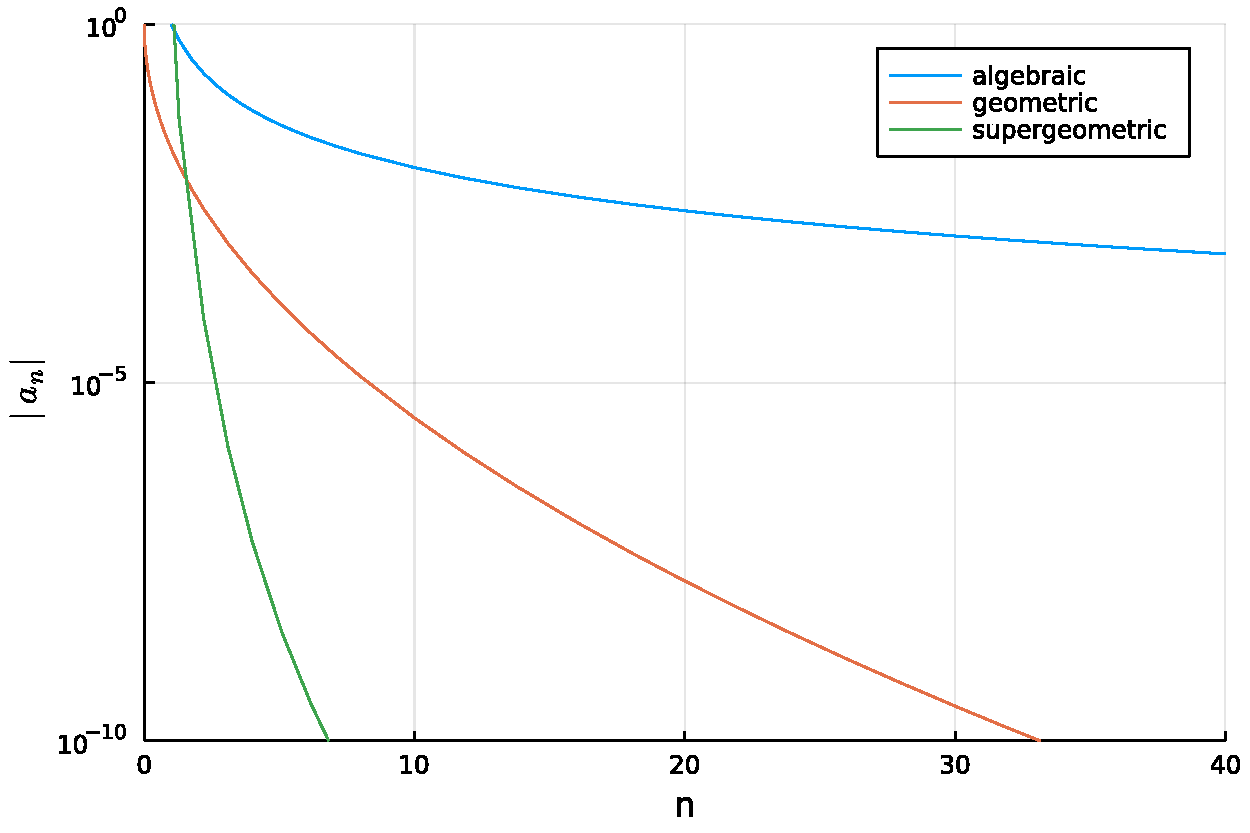
\includegraphics[keepaspectratio,scale = 0.35]{02_Fourier/typeoforder.pdf}
	\caption{Types of order}
\end{figure}

\subsubsection{その他の便利な性質}

- 微分
$$
    \frac{d}{dx} f(x) = \sum_{k=-\infty}^{\infty} (\im k)c_k e^{\im kx}
$$

- シフト
$$
    f(x-d) = \sum_{k=-\infty}^{\infty}c_ke^{\im k(x-d)} = \sum_{k=-\infty}^{\infty}(e^{-\im kd})c_ke^{\im kx}
$$

元の係数 $c_k$ に $ik$ や $e^{\im kd}$ を掛けるだけで演算ができる。
\end{comment}
%%

\subsection{フーリエ係数の計算方法}

周期関数 $f(x)$ のフーリエ係数 $c_k$ を数値計算で求めることを考える。フーリエ係数の添字のサイズ $N$ を $|k|<N$ となるように定める($N-1$ を最大波数ともいう)。

このとき、$0 = x_0\le x_1\le \dots \le x_{2N-1}=2\pi$ と区間 $[0,2\pi]$ を等間隔に分割した点 $x_j = jh$ ($j = 0,\dots,2N-1$, $h=2\pi/(2N-1)$) を標本点といい、標本点上での関数値を用いて次のようなフーリエ係数の近似を得る。

\begin{align*}
c_k &= \frac{1}{2\pi}\int_0^{2\pi}f(x)e^{-\im k x}dx \\
& \approx \frac1{2N-1}\sum_{j=0}^{2N-2} f(x_j) e^{-2\pi \im\frac{kj}{2N-1}}=\bar{c}_k,\quad (|k|<N).
\end{align*}

この $\bar{c}_k$ の式は、離散フーリエ変換の式 ($ a_k = \mathcal{F}_k(b) = \sum_{j=0}^{2M-2}b_j e^{-2\pi \im \frac{jk}{2M-1}}$) を用いて、高速フーリエ変換(FFT)で実装することができる。そして、近似されたフーリエ係数 $\bar{c}_k$ を使って、元の関数 $f(x)$ の近似が
$$
f^{(N)}(x) = \sum_{|k|<N} \bar{c}_k e^{\im k x}
$$
と得られる。

\subsection{フーリエ係数から元の関数の概形を求める}

関数 $f^{(N)}(x)$ の係数 $\bar{c}_k$ から元の関数をプロットしたい。いま標本点上での関数値は
$$
f^{(N)}(x_j) = \sum_{|k|<N} \bar{c}_k e^{\im k x_j} = \sum_{|k|<N} \bar{c}_k e^{2\pi\im \frac{kj}{2N-1}}.
$$

これは逆離散フーリエ変換に相当する。そこで逆高速フーリエ変換(IFFT)を用いて元の関数を求める。しかし、このままIFFTを用いると、標本点と同じ数の関数値しか得られず、グラフに描画すると粗くになってしまう。これを解消するために、フーリエ係数 $\bar{c}_k$ に $0$ を余分に貼り合わせて (paddingという) 、滑らかなグラフを得る。

\subsection{周期が $2\pi$ 以外の場合の取り扱い方}

$f(t)$ を周期 $L$ の周期関数とする。このとき変数 $t:a\to b$ ($L=b-a$) に対して、変数 $x$ を $x = \omega(t-a)$ ($\omega = 2\pi/L$) と定めると、$x:0\to 2\pi$ となり、関数 $g(x)\equiv f(a + \omega^{-1} x)$ は周期 $2\pi$ の周期関数である。

いま $g(x)$ がフーリエ級数
$$
g(x) = \sum_{k \in \mathbb{Z}} c_k e^{\im k x}
$$
で表されているとすると、
$$
f(t) = g(\omega (t-a)) = \sum_{k \in \mathbb{Z}} c_k e^{\im k \omega (t-a)},% = \sum_{k \in \mathbb{Z}} d_k e^{\im k \omega t},\quad d_k = e^{-\im k \omega a}c_k
$$
が成り立つ。フーリエ係数 $(c_k)_{k\in\mathbb{Z}}$ は
$$
c_k  = \frac{1}{2 \pi} \int_0 ^{2\pi} g(x) e^{-\im k x} dx = \frac{1}{L} \int_a ^b f(t) e^{-\im k \omega (t-a)} dt
$$
となり、$(c_k)_{k\in\mathbb{Z}}$ は次のように近似される。
$$
c_k \approx \frac{1}{2N-1} \sum_{j=0}^{2N-2} f(t_j) e^{-2 \pi \im \frac{kj}{2N-1}}.
$$

ここで、$t_j = a + \frac{jL}{2N-1}$ ($j=0,1,\dots,2N-2$) このことから、周期が $2\pi$ の周期関数とフーリエ係数の近似が同じ式になるため、フーリエ係数の計算方法は、先程と変わらない。

%\end{document}